\subsection{Selektion}
Som tidligere diskuteret er processen for genetiske algoritmer følgende:

•	Forældre individerne bliver valgt.


•	Forældrene parres.


•	Populationen vokser.


•	Individerne bliver muteret, eller krydset.


•	Sandsynligheden for at en crossover eller mutation finder sted bliver bestemt ud fra en selektionsmetode.


I det følgende afsnit beskrives nogle af de selektionsmetoder der kan bruges. Det vil endvidere også blive diskuteret, hvilken af disse metoder der bedst kan anvendes til at producere skoleskemaer.\footfullcite{winston2014}

\subsubsection{Roulette metoden}

Man kan forestille sig at hvert individ er tildelt et stykke på en roulette og størrelsen på stykket er proportional med individets fitness. Roulette bliver spinnet n antal gange, det vil tage for at vælge forældrene til den næste generation. Under hvert spin bliver individet under roulettens markør valgt til, at være en del af en gruppe af forældre til den næste generation. En kandidat kan godt blive valgt til, at være forældre flere gange, da det er forældrene til næste generation og ikke selve individerne i generationen, der bliver valgt, gør det dog ingen forskel. Formålet med denne metode er, at få valgt de forældre med den største fitness til næste generation, da de har større sandsynlig for, at skabe individer med større fitness. Problemet med denne metode er dog, at den genetiske algoritme hurtigt vil stå fast i den ene del af fitness rummet, da det er muligt at vælge den samme forældre flere gange, og derved kan der blive skabt en meget ensartet population, som gør at der kun vil blive udforsket et bestemt område af rummet i stedet for at udforske hele rummet.\footfullcite{jebari2013}\footfullcite{selection}
Roulette metoden kan illustreres på følgende måde:
\begin{figure}[!h]
  \centering
  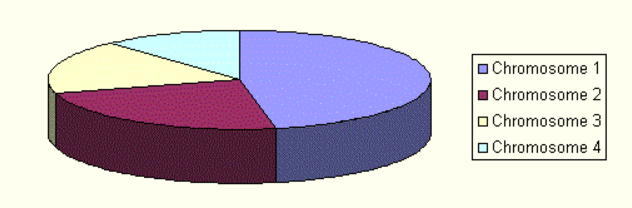
\includegraphics[width=\textwidth]{partials/graphics/roulette.png}
  \caption{Model over roulette metoden\footfullcite{roulette}.}
  \label{fig:roulette}
\end{figure}

\subsubsection{Rank metoden}

I rang metoden bliver individerne sorteret efter størrelsen på deres fitness. Derefter bliver individerne tildelt lodder efter den plads de har fået efter sorteringen. Det vil sige at den med den laveste fitness får tildelt et lod, den med den anden mindste får tildelt to lodder osv. Antallet af lodder et individ er blevet tildelt forstørre chancen for at individet bliver valgt som forældre til en fremtidig generation. I modsætning til roulette metoden, har fitnessen altså i rang metoden en indirekte påvirkning på individernes chance for at bliver valgt.\footfullcite{jebari2013} 

\subsubsection{Tournament metoden}

2 tilfældige individer bliver valgt fra populationen. Man generer en tilfældig værdi fra 0-1 for at sammenligne den med valgte sandsynlighedsværdi. Hvis værdien er mindre eller lige med sandsynlighedsværdien bliver det individ med højst fitness valgt ellers bliver individet med den lavere fitness valgt. Sandsynlighedsværdien bliver altid sat højere end 0.5 for at favorisere individet med den højeste fitness\footfullcite{jebari2013}. 

I det følgende program benyttes roulette metoden. Ved brug af roulette metoden sikres det at der er større sandsynlighed for at individerne med den højeste fitness bliver brugt til at skabe de fremtidige generationer. 

\subsection{Produktafgrænsning}
  Ved vores interview med Søren Kusk fra Sofiendalskolen, har vi fået information om, hvilke krav de stiller, når der ligges skema på Sofiendalskolen. Samt hvilke problemer der opstår under skolens skemalægning. Derudover er det blevet undersøgt hvorfor der bruges manuel skemalægning fremfor at bruge en af et allerede eksisterende softwareløsninger på markedet.
Ud fra vores empiri fra interviewet samt egen research af state of art, har vi fundet ud af, at de eksisterende skemaplanlægningsprogrammerne på markedet har svært ved at tage hensyn til folkeskoleskema, sådan lærere har tidsmæssigt samlede forberedelsestimer.
. På sofiendalskolen føler de at det vil være nødvendigt, at indgå kompromiser, og det er svært at standardiserer vigtigheden af de enkelte parametre der skal tages højde for i skemaplanlægningsprocessen. Derudover er det en tidskrævende proces for lærerne, at sætte sig ind og få forståelse for et af de allerede eksisterende skemaplanlægningsprogram\cite{interview}.
Ud fra denne viden, har vi besluttet at lave et program der kan lave et grundskema, der stemmer overens med de lovgivningsmæssige krav for elevernes timetal. Vores skema skal tage højde for at hver klasse og lærer ikke kan have mere end en lektion af gangen, samt et begrænset antal faglokaler. Vi vil ved brug af generisk algoritme lave et fit niveau der tilpasses af, i hvor høj grad det lykkedes at lægge lærernes forberedelsestimer i forlængelse af hinanden, så de har 2-3 timers forberedelse af gangen, fremfor mange små forberedelsestimer, da dette vægter højt for Sofiendalskolen.
Så vores program vil løse en del af det tidsmæssige problem for lærerne samt problemet med fordelte forberedelsestimer.

\subsection{Kravspecifikationer}
  Hvilke krav og bindinger skal vægtes i programmet:


•	Programmet skal generere skemaer for 9 klasser, 3 skemaer for henholdsvis 7, 8 og 9 klassetrin.


•	Programmet skal overholde minimumskravene for timetal i folkeskolen.


•	Programmet skal tage højde for at klassetrinene ikke har det samme antal fag eller samme type fag.


•	Det skal ikke være muligt for en lærer at have lektioner i to klasser på en gang.


•	Lærerne skal have mere end en forberedelsestime adgangen.


•	Der må ikke være tomme lektioner i midten eller starten af skemaet.


•	Samarbejde på tværs af parallelklasserne skal være muligt. 


•	Programmet skal læse lærernes initialer ind via en fil. Filen skal simulere en indstillingsmenu for forbrugeren.


•	Der må højest være 8 lektioner på en dag.


•	Lektionerne skal helst være ligeligt fordelt over alle ugedagene, således at der ikke er 3 dage med 8 lektioner og 2 dage med 4 lektioner.


\subsection{Selektion}
  I programmet anvendes en række defines i toppen, hvor værdierne kan ændres efter behov. Så er de forskellige skolefag skrevet som en enumeration type, efterfulgt af definitioner på de anvendte structs. Herefter ligger alle anvendte funktioner som prototyper. Selve funktionerne ligger i bunden. Kommentarer skrives over det stykke kode den forklarer. Når der udføres en algoritme i en funktion eller en løkke, er algoritmen rykket ind med et tab af to mellemrum. Tuborgklammer starter inden linjeskift, efter funktioner og løkker, og afsluttes efter et linjeskift. 